\section{Results}
\label{sec:results}

\paragraph{Family-conditional hardness (completed bench).}
On the fitted DenoiseOpt 100\,000-cycle bench, denoise score $D$ is lowest for \texttt{nonlinear} ($D\approx 0.39$) and \texttt{combo} ($D\approx 0.40$), then \texttt{triple\_mix} / \texttt{extreme\_overlay} ($D\approx 0.51$--$0.52$), while \texttt{harmonic\_fft} and \texttt{am\_fm} sit near $D\approx 0.69$--$0.70$.
Lit-combo champion family stress (prolonged residual) similarly ranks \texttt{open\_wrap\_bias} ($R\approx 0.83$) and \texttt{extreme\_overlay} / \texttt{combo} ($R\approx 0.88$--$0.89$) below \texttt{harmonic\_fft} ($R\approx 0.95$).
Hard sounds recur; they are not a random one-off.

\paragraph{Overnight hybrid (interim).}
Final mean-$R$ tables will be ingested after the overnight campaign reaches its declared iteration budget.
Monitoring plots below are for protocol transparency only; incomplete-run champions are \emph{not} asserted as finished science.

\begin{figure}[t]
  \centering
  
\includegraphics[width=\columnwidth]{figures/champ_residual_vs_iter.png}
  \caption{Interim champion residual $R$ versus search iteration, with DualCosine baseline. Monitoring snapshot; not a final result.}
  \label{fig:champ-residual}
\end{figure}

\begin{figure}[t]
  \centering
  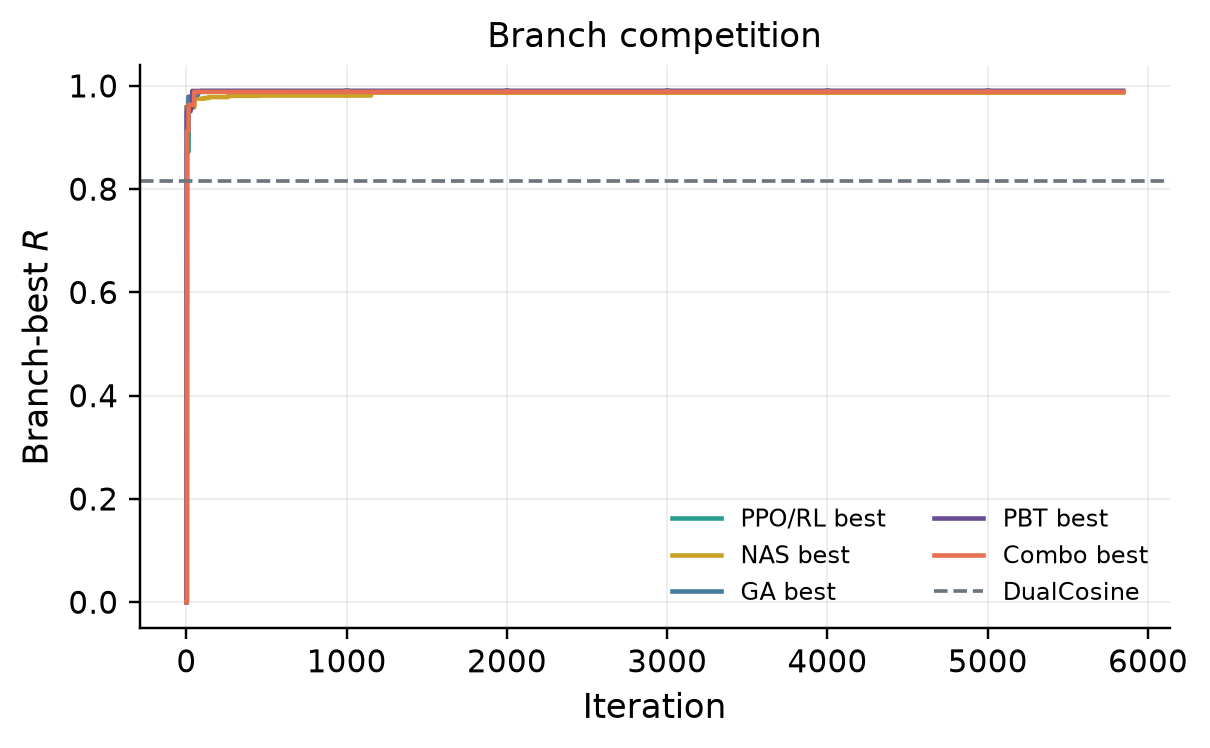
\includegraphics[width=\columnwidth]{figures/branch_bests_vs_iter.png}
  \caption{Interim per-branch best residual trajectories (PPO/RL, GA, PBT, NAS, combo). Monitoring only.}
  \label{fig:branch-bests}
\end{figure}

\begin{figure*}[t]
  \centering
  
\includegraphics[width=\textwidth]{figures/overnight_panel.png}
  \caption{Full-width interim overnight monitoring panel: champion $R$ (top) and branch-best trajectories (bottom). Snapshot while the GPU budget completes.}
  \label{fig:overnight-panel}
\end{figure*}

\begin{figure}[t]
  \centering
  
\includegraphics[width=\columnwidth]{figures/residual_by_branch.png}
  \caption{Interim per-trial residual scatter by search branch, with champion overlay. Monitoring snapshot.}
  \label{fig:residual-branch}
\end{figure}

\begin{figure}[t]
  \centering
  
\includegraphics[width=\columnwidth]{figures/champion_timeline.png}
  \caption{Interim champion update timeline. Sparse $R$ labels mark first, peak-mid, and latest improvements to stay legible in twocolumn.}
  \label{fig:champ-timeline}
\end{figure}
